\section{Using derivatives to identify extreme values of a function} \label{S:3.2.Tests}

\begin{goals}
\item What are the critical values of a function $f$ and how are they connected to identifying the most extreme values the function achieves?
\item How does the first derivative of a function reveal important information about the behavior of the function, including the function's extreme values?
\item How can the second derivative of a function be used to help identify extreme values of the function?
\end{goals}

%--------------------------------------
% SUBSECTION INTRODUCTION
%--------------------------------------
\subsection*{Introduction}

In many different settings, we are interested in knowing where a function achieves its least and greatest values.  These can be important in applications -- say to identify a point at which maximum profit or minimum cost occurs -- or in theory to understand how to characterize the behavior of a function or a family of related functions.  Consider the simple and familiar example of a parabolic function such as $s(t) = -16t^2 + 32t + 48$ (shown at left in Figure~\ref{fig:3.2.Intro}) that represents the height of an object tossed vertically:  its maximum value occurs at the vertex of the parabola and represents the highest value that the object reaches.  Moreover, this maximum value identifies an especially important point on the graph, the point at which the curve changes from increasing to decreasing.

\begin{marginfigure}[1cm] % MARGIN FIGURE
\margingraphics{figures/3_1_Intro.eps}
\caption{At left, $s(t) = -16t^2 + 24t + 32$ whose vertex is $(\frac{3}{4}, 41)$; at right, a function $g$ that demonstrates several high and low points.} \label{fig:3.2.Intro}
\end{marginfigure}

More generally, for any function we consider, we can investigate where its lowest and highest points occur in comparison to points nearby or to all possible points on the graph.  Given a function $f$, we say that $f(c)$ is a \emph{global} or \emph{absolute maximum}  \index{maximum!global} \index{maximum!absolute} provided that $f(c) \ge f(x)$ for all $x$ in the domain of $f$, and similarly call $f(c)$ a \emph{global} \index{minimum!global} or \emph{absolute minimum} \index{minimum!absolute} whenever $f(c) \le f(x)$ for all $x$ in the domain of $f$.  For instance, for the function $g$ given at right in Figure~\ref{fig:3.2.Intro}, $g$ has a global maximum of $g(c)$, but $g$ does not appear to have a global minimum, as the graph of $g$ seems to decrease without bound.  We note that the point $(c,g(c))$ marks a fundamental change in the behavior of $g$, where $g$ changes from increasing to decreasing; similar things happen at both $(a,g(a))$ and $(b,g(b))$, although these points are not global mins or maxes.  

For any function $f$, we say that $f(c)$ is a \emph{local maximum} \index{maximum!local} or \emph{relative maximum} \index{maximum!relative} provided that $f(c) \ge f(x)$ for all $x$ near $c$, while $f(c)$ is called a \emph{local} \index{minimum!local} or \emph{relative minimum} \index{minimum!relative} whenever $f(c) \le f(x)$ for all $x$ near $c$.  Any maximum or minimum may be called an \emph{extreme value} \index{extreme value} of $f$.  For example, in Figure~\ref{fig:3.2.Intro}, $g$ has a relative minimum of $g(b)$ at the point $(b,g(b))$ and a relative maximum of $g(a)$ at $(a,g(a))$.  We have already identified the global maximum of $g$ as $g(c)$; this global maximum can also be considered a relative maximum.  

We would like to use fundamental calculus ideas to help us identify and classify key function behavior, including the location of relative extremes.  Of course, if we are given a graph of a function, it is often straightforward to locate these important behaviors visually.  We investigate this situation in the following preview activity.

\begin{marginfigure}[6cm]
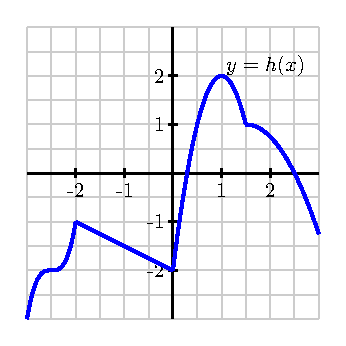
\includegraphics{figures/3_1_PA1.eps}
\caption{The graph of a function $h$ on the interval $[-3,3]$.} \label{fig:3.1.PA1}
\end{marginfigure}

\begin{pa} \label{PA:3.1}
Consider the function $h$ given by the graph in Figure~\ref{fig:3.1.PA1}.  Use the graph to answer each of the following questions.

\ba
	\item Identify all values $c$ for which $h(c)$ is a local maximum of $h$.
	\item Identify all values $c$ for which $h(c)$ is a local minimum of $h$.
	\item Does $h$ have a global maximum?  If so, what is the value of this global maximum?
	\item Does $h$ have a global minimum?  If so, what is its value?
	\item Identify all values of $c$ for which $h'(c) = 0$.
	\item Identify all values of $c$ for which $h'(c)$ does not exist.
	\item True or false: every relative maximum and minimum of $h$ occurs at a point where $h'(c)$ is either zero or does not exist.
	\item True or false: at every point where $h'(c)$ is zero or does not exist, $h$ has a relative maximum or minimum.
\ea
\end{pa} \afterpa % PREVIEW ACTIVITY

%-------------------------------------------------------
% SUBSECTION INCREASING/DECREASING TEST
%-------------------------------------------------------
\subsection*{Increasing/Decreasing test}

Before we continue examining extreme values of a function, let's recall a topic we discussed that we will use throughout this section.
In Section~\ref{S:2.3.SecondD}, we discussed that whether a function is increasing or decreasing depends precisely on the value of the derivative at a point. Repeating the idea here, a function is increasing at $x=a$ if and only if $f'(a)>0$ and decreasing at $x=a$ if and only if $f'(a)<0$. This can be expanded to intervals in the domain of the function which we state in the following concept.

\concept{Test for Increasing/Decreasing Functions} % CONCEPT
{Let $f$ be a continuous function on $[a,b]$ and differentiable on $(a,b)$.
\begin{enumerate}
\item If $f'(c) > 0$ for all $c$ in $(a,b)$, then $f$ is increasing on $[a,b]$.
\item If $f'(c) <0$ for all $c$ in $(a,b)$, then $f$ is decreasing on $[a,b]$.
\item If $f'(c) =0$ for all $c$ in $(a,b)$, then $f$ is constant on $[a,b]$.
\end{enumerate}
} %end concept

If $f'(x)=0$ for a finite number of $x$ values as oppossed to the entire interval $(a,b)$\footnote{If $f$ is constant on $[a,b]$, then the graph of $f$ is a horizontal line and therefore its rate of change is $0$ for values in $(a,b)$.}, the function is neither increasing or decreasing at those values.  The values where $f'(x)= 0$ are very important in identifying extreme values and require more examination.

%-----------------------------------------------------------------------------------
% SUBSECTION CRITICAL VALUES AND THE FIRST DERIVATIVE TEST
%-----------------------------------------------------------------------------------
\subsection*{Critical values and the first derivative test}
 
If a function has a relative extreme value at a point $(c,f(c))$, the function must change its behavior at $c$ regarding whether it is increasing or decreasing before or after the point.

\begin{figure*} % FIGURE
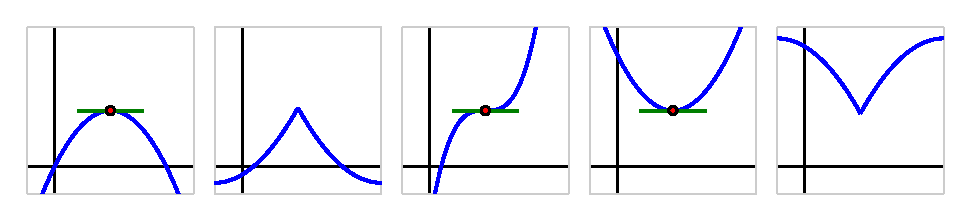
\includegraphics{figures/3_1_extremes.eps}
\caption{From left to right, a function with a relative maximum where its derivative is zero; a function with a relative maximum where its derivative is undefined; a function with neither a maximum nor a minimum at a point where its derivative is zero; a function with a relative minimum where its derivative is zero; and a function with a relative minimum where its derivative is undefined.} \label{fig:3.2.extremes}
\end{figure*} 

For example, if a continuous function has a relative maximum at $c$, such as those pictured in the two leftmost functions in Figure~\ref{fig:3.2.extremes}, then it is both necessary and sufficient that the function change from being increasing just before $c$ to decreasing just after $c$.  In the same way, a continuous function has a relative minimum at $c$ if and only if the function changes from decreasing to increasing at $c$.  See, for instance, the two functions pictured at right in Figure~\ref{fig:3.2.extremes}.  There are only two possible ways for these changes in behavior to occur:  either $f'(c) = 0$ or $f'(c)$ is undefined.  

Because these values of $c$ are so important, we call them \emph{critical values}.  More specifically, we say that a function $f$ has a \emph{critical value} \index{critical value} at  $x = c$ provided that $f'(c) = 0$ or $f'(c)$ is undefined.   Critical values provide us with the only possible locations where the function $f$ may have relative extremes.  Note that not every critical value produces a maximum or minimum; in the middle graph of Figure~\ref{fig:3.2.extremes}, the function pictured there has a horizontal tangent line at the noted point, but the function is increasing before and increasing after, so the critical value does not yield a location where the function is greater than every value nearby, nor less than every value nearby.

The \emph{first derivative test} \index{first derivative test} summarizes how sign changes in the first derivative indicate the presence of a local maximum or minimum for a given function.

\concept{First Derivative Test\index{first derivative test}} { % CONCEPT
If $p$ is a critical value of a continuous function $f$ that is differentiable near $p$ (except possibly at $x = p$), then $f$ has a relative maximum at $p$ if and only if $f'$ changes sign from positive to negative at $p$, and $f$ has a relative minimum at $p$ if and only if $f'$ changes sign from negative to positive at $p$.
} % end concept

We consider an example to show one way the first derivative test can be used to identify the relative extreme values of a function.

\begin{marginfigure}[8cm]
\margingraphics{figures/3_1_signchart.eps} %Active ex3.1 
\caption{The first derivative sign chart for a function $f$ whose derivative is given by the formula $f'(x) = e^{-2x}(3-x)(x+1)^2$.} \label{fig:3.2.signchart}
\end{marginfigure}

\begin{example} \label{Ex:3.2.Eg1}
Let $f$ be a function whose derivative is given by the formula $f'(x) = e^{-2x}(3-x)(x+1)^2$.  Determine all critical values of $f$ and decide whether a relative maximum, relative minimum, or neither occurs at each.

\solution Since we already have $f'(x)$ written in factored form, it is straightforward to find the critical values  of $f$.  Since $f'(x)$ is defined for all values of $x$, we need only determine where $f'(x) = 0$.  From the equation
$$e^{-2x}(3-x)(x+1)^2 = 0$$
and the zero product property, it follows that $x = 3$ and $x = -1$ are critical values of $f$.  (Note particularly that there is no value of $x$ that makes $e^{-2x} = 0$.)  

Next, to apply the first derivative test, we'd like to know the sign of $f'(x)$ at values near the critical values.  Because the critical values are the only locations at which $f'$ can change sign, it follows that the sign of the derivative is the same on each of the intervals created by the critical values:  for instance, the sign of $f'$ must be the same for every value of $x < -1$.  We create a first derivative sign chart to summarize the sign of $f'$ on the relevant intervals along with the corresponding behavior of $f$.

The first derivative sign chart in Figure~\ref{fig:3.2.signchart} comes from thinking about the sign of each of the terms in the factored form of $f'(x)$ at one selected point in the interval under consideration.  For instance, for $x < -1$, we could consider $x = -2$ and determine the sign of $e^{-2x}$, $(3-x)$, and $(x+1)^2$ at the value $x = -2$.  We note that both $e^{-2x}$ and $(x+1)^2$ are positive regardless of the value of $x$, while $(3-x)$ is also positive at $x = -2$.  Hence, each of the three terms in $f'$ is positive, which we indicate by writing ``$+++$.''  Taking the product of three positive terms obviously results in a value that is positive, which we denote by the ``$+$'' in the interval to the left of $x = -1$ indicating the overall sign of $f'$.  And, since $f'$ is positive on that interval, we further know that $f$ is increasing, which we summarize by writing ``INC'' to represent the corresponding behavior of $f$.  In a similar way, we find that $f'$ is positive and $f$ is increasing on $-1 < x < 3$, and $f'$ is negative and $f$ is decreasing for $x > 3$.

Now, by the first derivative test, to find relative extremes of $f$ we look for critical value at which $f'$ changes sign.  In this example, $f'$ only changes sign at $x = 3$, where $f'$ changes from positive to negative, and thus $f$ has a relative maximum at $x = 3$.  While $f$ has a critical value at $x = -1$, since $f$ is increasing both before and after $x = -1$, $f$ has neither a minimum nor a maximum at $x = -1$.
\end{example} % EXAMPLE

\begin{marginfigure}[4cm]
\margingraphics{figures/figincr2} %APEX ex85 p.138
\caption{A graph of $f(x)$ and $f'(x)$ in Example~\ref{Ex:3.2.Eg2}, showing where $f$ is increasing and decreasing.} \label{fig:eg3.2.graph}
\end{marginfigure}

\begin{marginfigure}[4cm]
\margingraphics{figures/figincrline2} %APEX ex85 p.138
\caption{Number line for $f$ in Example \ref{Ex:3.2.Eg2}.}
\label{F:3.2.signchart}
\end{marginfigure}

\begin{example} \label{Ex:3.2.Eg2}
Find the intervals on which $f$ is increasing and decreasing, and use the First Derivative Test to determine the relative extrema of $f$, where 
$$f(x) = \frac{x^2+3}{x-1}.$$

\solution We start by calculating $\fp$ using the Quotient Rule. We find
$$\fp(x) = \frac{x^2-2x-3}{(x-1)^2}.$$
We need to find the critical values of $f$; we want to know when $\fp(x)=0$ and when $\fp$ is not defined. That latter is straightforward: when the denominator of $\fp$ is $0$, $\fp$ is undefined. That occurs when $x=1$. $\fp(x)=0$ when the numerator of $\fp$ is $0$. That occurs when $x^2-2x-3 = (x-3)(x+1) = 0$; i.e., when $x=-1,3$. 

We have found that $f$ has three critical numbers, dividing the real number line into $4$ subintervals: $$(-\infty,-1), \quad (-1, 1), \quad (1,3) \quad \text{and} \quad (3,\infty).$$ Pick a number $p$ from each subinterval and test the sign of \fp\ at $p$ to determine whether $f$ is increasing or decreasing on that interval. Again, we do well to avoid complicated computations; notice that the denominator of $\fp$ is \textit{always} positive so we can ignore it during our work.\\

\noindent\textbf{Interval 1}, $(-\infty,-1)$:\quad  Choosing a very small number (i.e., a negative number with a large magnitude) $p$ returns $p^2-2p-3$ in the numerator of $\fp$; that will be positive. Hence $f$ is increasing on $(-\infty,-1)$.\\

\noindent\textbf{Interval 2}, $(-1,1)$:\quad Choosing $0$ seems simple: $\fp(0)=-3<0$. We conclude $f$ is decreasing on $(-1,1)$.\\

\noindent\textbf{Interval 3}, $(1,3)$:\quad Choosing $2$ seems simple: $\fp(2) = -3<0$. Again, $f$ is decreasing.\\

\noindent \textbf{Interval 4}, $(3,\infty)$:\quad	Choosing a very large number $p$ from this subinterval will give a positive numerator and (of course) a positive denominator. So $f$ is increasing on $(3,\infty)$.\\

In summary, $f$ is increasing on the set $(-\infty,-1)\cup (3,\infty)$ and is decreasing on the set $(-1,1)\cup (1,3)$. Since at $x=-1$, the sign of $\fp$ switched from positive to negative, then $f(-1)$ is a relative maximum of $f$. At $x=3$, the sign of $\fp$ switched from negative to positive, meaning $f(3)$ is a relative minimum. At $x=1$, $f$ is not defined, so there is no relative extrema at $x=1$.
 
This is summarized in the number line shown in Figure \ref{F:3.2.signchart}. Also, Figure \ref{fig:eg3.2.graph} shows a graph of $f$, confirming our calculations. This figure also shows $\fp$ in red, again demonstrating that $f$ is increasing when $\fp>0$ and decreasing when $\fp<0$.

%\centering
%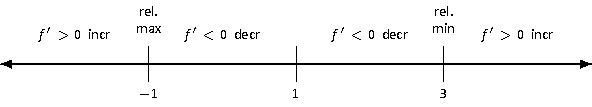
\includegraphics{figures/figincrline2}
%\captionsetup{type=figure}%
%\caption{Number line for $f$ in Example \ref{ex_incr2}.}\label{fig:incrline2}
\end{example} % EXAMPLE

\begin{activity} \label{A:3.2.1}  Suppose that $g(x)$ is a function continuous for every value of $x \ne 2$ whose first derivative is $\ds g'(x) = \frac{(x+4)(x-1)^2}{x-2}$.  Further, assume that it is known that $g$ has a vertical asymptote at $x = 2$.
\ba
  \item Determine all critical values of $g$.
  \item By developing a carefully labeled first derivative sign chart, decide whether $g$ has  as a local maximum, local minimum, or neither at each critical value.
  \item Does $g$ have a global maximum? global minimum? Justify your claims.
  \item What is the value of $\ds \lim_{x \to \infty} g'(x)$?  What does the value of this limit tell you about the long-term behavior of $g$?
  \item Sketch a possible graph of $y = g(x)$.
\ea
\end{activity}
\begin{smallhint}
\ba
	\item For which $x$ is $g'(x) = 0$?
	\item Note that $(x-1)^2$ is positive for all $x \ne 1$.
	\item Use your first derivative sign chart from (b).
	\item Try expanding the numerator before evaluating the limit.
	\item Think carefully about the information from the sign chart found in (b).
\ea
\end{smallhint}
\begin{bighint}
\ba
	\item For which $x$ is $g'(x) = 0$?  Remember that a fraction's value is zero if and only if its numerator is zero.
	\item Note that $(x-1)^2$ is positive for all $x \ne 1$.  How do the signs of $(x+4)$ and $(x-2)$ then determine the overall sign of $g'(x)$?
	\item Use your first derivative sign chart from (b) and remember to the first derivative test.
	\item Try expanding the numerator before evaluating the limit and think about what you know about the limit of a rational function as $x \to \infty$.
	\item Focus on where $g$ is increasing and decreasing, along with where it must have a horizontal tangent line.
\ea
\end{bighint}
\begin{activitySolution}
\ba
  \item Since $\ds g'(x) = \frac{(x+4)(x-1)^2}{x-2}$, we see that $g'(x) = 0$ implies that $x = -4$ or $x = 1$.  While $x = 2$ makes $g'$ undefined, we are told that $g$ has a vertical asymptote at $x = 2$, so $x = 2$ is not in the domain of $g$, and hence is technically not a critical value of $g$.  Nonetheless, we place $x = 2$ on our first derivative sign chart since the vertical asymptote is a location at which $g'$ may change sign.
  \item The first derivative sign chart shows that $g'(x) > 0$ for $x < -4$, $g'(x) < 0$ for $-4 < x < 1$, $g'(x) < 0$ for $1 < x < 2$, and $g'(x) > 0$ for $x > 2$.  By the first derivative test, $g$ has a local maximum at $x = -4$ and neither a max nor min at $x = 1$.  As these are the only two critical values, these are the only two locations for possible extremes.  (Note: although $g$ changes from decreasing to increasing at $x = 2$, this is due to a vertical asymptote, and $g$ does not have a minimum there.)
  \item Because $g$ is decreasing as $x \to 2^-$ (where $g$ has a vertical asymptote), $g$ does not have a global minimum.  For $x > 2$, $g$ is always increasing, which suggests that $g$ does not have a global maximum (though we do not know for sure that $g$ increases without bound).
  \item We observe that
  \begin{eqnarray*} 
  	\lim_{x \to \infty} g'(x) & = & \lim_{x \to \infty} \frac{(x+4)(x-1)^2}{x-2} \\
					& = & \lim_{x \to \infty} \frac{x^3 + 2x^2 - 7x + 4}{x-2} \cdot \frac{\frac{1}{x}}{\frac{1}{x}} \\
					& = & \lim_{x \to \infty} \frac{x^2 + 2x - 7 + \frac{4}{x}}{1 - \frac{2}{x}} \\
					& = & \infty
  \end{eqnarray*}
Since $g'(x) \to \infty$ as $x \to \infty$, this tells us that $g$ increases without bound as $x \to \infty$.
  \item From all of our work above, we know that $g$ has a local maximum at $x = -4$, a horizontal tangent line with neither a max nor min at $x = 1$, and a vertical asymptote at $x = 2$, plus $g$ and $g'$ both increase without bound as $x \to \infty$.  Thus, a possible graph of $g$ is the following.
  \begin{center}
  	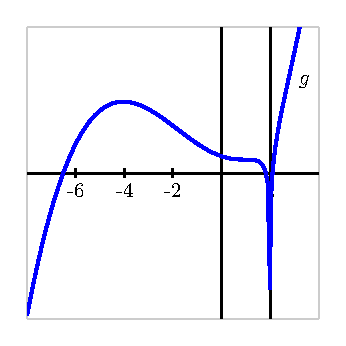
\includegraphics{figures/3_1_Act1Soln.eps}
  \end{center}
\ea
\end{activitySolution}
\aftera % ACTIVITY

%---------------------------------------------------------
% SUBSECTION THE SECOND DERIVATIVE TEST
%---------------------------------------------------------
\subsection*{The second derivative test}

Recall that the second derivative of a function tells us several important things about the behavior of the function itself.  For instance, if $f''$ is positive on an interval, then we know that $f'$ is increasing on that interval and, consequently, that $f$ is concave up,\footnote{See Section~\ref{S:2.3.SecondD} for the definition of concavity.} which also tells us that throughout the interval the tangent line to $y = f(x)$ lies below the curve at every point.  In this situation where we know that $f'(p) = 0$, it turns out that the sign of the second derivative determines whether $f$ has a local minimum or local maximum at the critical value $p$.

In Figure~\ref{fig:3.2.2Dtest}, we see the four possibilities for a function $f$ that has a critical point $p$ at which $f'(p) = 0$, provided $f''(p)$ is not zero on an interval including $p$ (except possibly at $p$).  On either side of the critical point, $f''$ can be either positive or negative, and hence $f$ can be either concave up or concave down.  In the first two graphs, $f$ does not change concavity at $p$, and in those situations, $f$ has either a local minimum or local maximum.  In particular, if $f'(p) = 0$ and $f''(p) < 0$, then we know $f$ is concave down at $p$ with a horizontal tangent line, and this guarantees $f$ has a local maximum there.  This fact, along with the corresponding statement for when $f''(p)$ is positive, is stated in the \emph{second derivative test}. 

\begin{figure*} % FIGURE
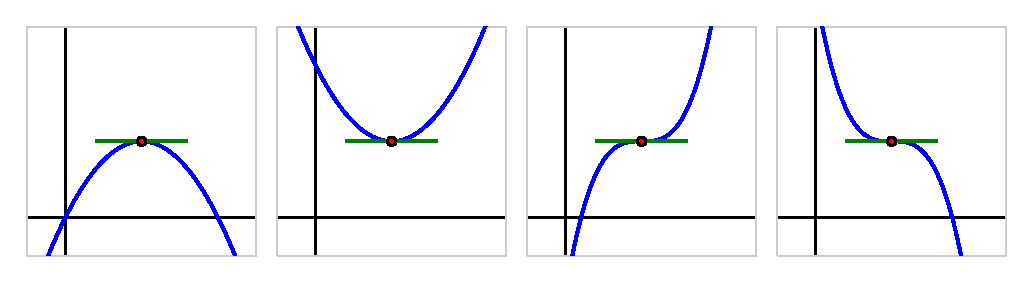
\includegraphics{figures/3_1_2Dtest.eps} %active p156
\caption{Four possible graphs of a function $f$ with a horizontal tangent line at a critical value.} \label{fig:3.2.2Dtest}
\end{figure*}

\concept{Second Derivative Test\index{second derivative test}} { %CONCEPT 
If $p$ is a critical value of a continuous function $f$ such that $f'(p) = 0$ and $f''(p) \ne 0$, then $f$ has a relative maximum at $p$ if and only if $f''(p) < 0$, and $f$ has a relative minimum at $p$ if and only if $f''(p) > 0$.
} % end concept

In the event that $f''(p) = 0$, the second derivative test is inconclusive.  That is, the test doesn't provide us any information.  This is because if $f''(p) = 0$, it is possible that $f$ has a local minimum, local maximum, or neither.\footnote{Consider the functions $f(x) = x^4$, $g(x) = -x^4$, and $h(x) = x^3$ at the critical point $p = 0$.}

Just as a first derivative sign chart reveals all of the increasing and decreasing behavior of a function, we can construct a second derivative sign chart that demonstrates all of the important information involving concavity.

\begin{marginfigure}[6cm]
\margingraphics{figures/3_1_signchart2.eps} %Active p.157
\caption{The first derivative sign chart for $f$ when $f'(x) = 3x^4 - 9x^2 = 3x^2(x^2-3)$ in Example \ref{Ex:3.2.Eg3}.}
\label{F:3.2.signchart2}
\end{marginfigure}

\begin{example} \label{Ex:3.2.Eg3}
Let $f(x)$ be a function whose first derivative is $f'(x) = 3x^4 - 9x^2$.  Construct both first and second derivative sign charts for $f$, fully discuss where $f$ is increasing and decreasing and concave up and concave down, identify all relative extreme values, and sketch a possible graph of $f$.

\solution Since we know $f'(x) = 3x^4 - 9x^2$, we can find the critical values of $f$ by solving $3x^4 - 9x^2 = 0$.  Factoring, we observe that
$$0 = 3x^2(x^2 - 3) = 3x^2(x+\sqrt{3})(x-\sqrt{3}),$$
so that $x = 0, \pm\sqrt{3}$ are the three critical values of $f$.  It then follows that the first derivative sign chart for $f$ is given in Figure~\ref{F:3.2.signchart2}.

Thus, $f$ is increasing on the intervals $(-\infty, -\sqrt{3})$ and $(\sqrt{3}, \infty)$, while $f$ is decreasing on $(-\sqrt{3},0)$ and $(0, \sqrt{3})$.  Note particularly that by the first derivative test, this information tells us that $f$ has a local maximum at $x = -\sqrt{3}$ and a local minimum at $x = \sqrt{3}$.  While $f$ also has a critical value at $x = 0$, neither a maximum nor minimum occurs there since $f'$ does not change sign at $x = 0$.

Next, we move on to investigate concavity.  Differentiating $f'(x) = 3x^4 - 9x^2$, we see that $f''(x) = 12x^3 - 18x$.  Since we are interested in knowing the intervals on which $f''$ is positive and negative, we first find where $f''(x) = 0$.  Observe that
$$0 = 12x^3 - 18x = 12x\left(x^2 - \frac{3}{2}\right) = 12x\left(x+\sqrt{\frac{3}{2}}\right)\left(x-\sqrt{\frac{3}{2}}\right),$$
which implies that $x = 0, \pm\sqrt{\frac{3}{2}}$.  Building a sign chart for $f''$ in the exact same way we do so for $f'$, we see the result shown in Figure~\ref{F:3.2.signchart3}.

Therefore, $f$ is concave down on the intervals $\left( -\infty, -\sqrt{\frac{3}{2}} \right)$ and $\left( 0, \sqrt{\frac{3}{2}} \right)$, and concave up on $\left( 0, \sqrt{\frac{3}{2}} \right)$ and $\left( \sqrt{\frac{3}{2}}, \infty \right)$.

Putting all of the above information together, we now see a complete and accurate possible graph of $f$ in Figure~\ref{F:3.2.Eg3}.  

The point $A = (-\sqrt{3}, f(-\sqrt{3}))$ is a local maximum, as $f$ is increasing prior to $A$ and decreasing after; similarly, the point $E = (\sqrt{3}, f(\sqrt{3}))$ is a local minimum.  Note, too, that $f$ is concave down at $A$ and concave up at $B$, which is consistent both with our second derivative sign chart and the second derivative test.  At points $B$ and $D$, concavity changes, as we saw in the results of the second derivative sign chart in Figure~\ref{F:3.2.signchart3}.  Finally, at point $C$, $f$ has a critical value with a horizontal tangent line, but neither a maximum nor a minimum occurs there since $f$ is decreasing both before and after $C$.  It is also the case that concavity changes at $C$.

While we completely understand where $f$ is increasing and decreasing, where $f$ is concave up and concave down, and where $f$ has relative extremes, we do not know any specific information about the $y$-coordinates of points on the curve.  For instance, while we know that $f$ has a local maximum at $x = -\sqrt{3}$, we don't know the value of that maximum because we do not know $f(-\sqrt{3})$.  Any vertical translation of our sketch of $f$ in Figure~\ref{F:3.2.Eg3} would satisfy the given criteria for $f$.
\end{example}

\begin{marginfigure}[-18cm]
\margingraphics{figures/3_1_signchart3.eps} %Active p.157
\caption{The second derivative sign chart for $f$ when $f'(x) = 3x^4 - 9x^2 = 3x^2(x^2-3)$ in Example \ref{Ex:3.2.Eg3}.}
\label{F:3.2.signchart3}
\end{marginfigure}

\begin{marginfigure}[-7cm]
\margingraphics{figures/3_1_Ex2.eps} %Active p.158
\caption{A possible graph of the function $f$ in Example \ref{Ex:3.2.Eg3}.}
\label{F:3.2.Eg3}
\end{marginfigure} % EXAMPLE

Points $B$, $C$, and $D$ in Figure~\ref{F:3.2.Eg3} are locations at which the concavity of $f$ changes.  We give a special name to any such point:  if $p$ is a value in the domain of a continuous function $f$ at which $f$ changes concavity, then we say that $(p,f(p))$ is an \emph{inflection point} \index{inflection point} of $f$.  Just as we look for locations where $f$ changes from increasing to decreasing at points where $f'(p) = 0$ or $f'(p)$ is undefined, so too we find where $f''(p) = 0$ or $f''(p)$ is undefined to see if there are points of inflection at these locations.

It is important at this point in our study to remind ourselves of the big picture that derivatives help to paint:  the sign of the first derivative $f'$ tells us \emph{whether} the function $f$ is increasing or decreasing, while the sign of the second derivative $f''$ tells us \emph{how} the function $f$ is increasing or decreasing. \pagebreak

\begin{marginfigure}
\margingraphics{figures/3_1_Act2.eps} 
\caption{The graph of $y = g''(x)$.} \label{F:3.1.Act2}
\end{marginfigure}

\begin{activity} \label{A:3.1.2}  Suppose that $g$ is a function whose second derivative, $g''$, is given by the following graph.

\ba 
  \item Find all points of inflection of $g$. 
  \item Fully describe the concavity of $g$ by making an appropriate sign chart.  
  \item Suppose you are given that $g'(-1.67857351) = 0$.  Is there is a local maximum, local minimum, or neither (for the function $g$) at this critical value of $g$, or is it impossible to say?  Why?
  \item Assuming that $g''(x)$ is a polynomial (and that all important behavior of $g''$ is seen in the given graph, what degree polynomial do you think $g(x)$ is?  Why?
\ea
\end{activity}
\begin{smallhint}
\ba 
  \item What must be true of $g''(x)$ at a point of inflection?
  \item Use the given graph to decide where $g''$ is positive and negative.
  \item What does the second derivative test say?
  \item Can you guess a formula for $g''(x)$ based on its graph?
\ea
\end{smallhint}
\begin{bighint}
\ba 
  \item At what points on the given graph does $g''(x)$ change sign?
  \item From the given graph, where is $g''(x) > 0$?  $g''(x) < 0$?
  \item What does the second derivative test say?  What is $g''(-1.67857351)$?
  \item Can you guess a formula for $g''(x)$ based on its graph?  Note that $g''$ appears to have a repeated root at $x = 2$.
\ea
\end{bighint}
\begin{activitySolution}
\ba 
  \item Based on the given graph of $g''$, the only point at which $g''$ changes sign is $x = -1$, and hence this is an inflection point of $g$. 
  \item Note that $g''(x) > 0$ for $x < -1$, $g''(x) < 0$ for $-1 < x < 2$, and $g''(x) < 0$ for $x > 2$.  This tells us that $g$ is concave up for $x < -1$, concave down for $-1 < x < 2$, and concave down for $x > 2$.
  \item Given that $g'(-1.67857351) = 0$, we know that $g$ has a horizontal tangent line at this critical value.  In addition, from the given graph of $g''$, we see that $g''( -1.67857351) > 0$ and observe that $g$ is concave up at $x$-values near $-1.67857351$.  By the second derivative test, $g$ has a local minimum at $x = -1.67857351$.
  \item From the given graph, since $g''$ has a simple zero at $x = -1$ and a repeated zero at $x = 2$, it appears that $g''$ is a degree 3 polynomial.  If so, then $g'$ is a degree 4 polynomial, and $g$ is a degree 5 polynomial.
\ea
\end{activitySolution}
\aftera % ACTIVITY

We end this section with an application problem to help us better understand inflection points.

\begin{marginfigure}[2cm]
\margingraphics{figures/figconc3} %APEX ex89 p.145
\caption{A graph of $S(t)$ in Example \ref{Ex:3.2.Eg4}, modeling the sale of a product over time. }
\label{F:3.2.Eg4}
\end{marginfigure}

\begin{marginfigure}[0cm]
\margingraphics{figures/figconc3b} %APEX ex89 p.145
\caption{A graph of $S(t)$ and $S'(t)$ in Example~\ref{Ex:3.2.Eg4}.}
\label{F:3.2.Eg4b}
\end{marginfigure}

\begin{example} \label{Ex:3.2.Eg4}
The sales of a certain product over a three-year span are modeled by $S(t)= t^4-8t^2+20$, where $t$ is the time in years, shown in Figure \ref{F:3.2.Eg4}.  Over the first two years, sales are decreasing.  Find the point at which sales are decreasing at their greatest rate.

\solution We want to maximize the rate of decrease, which is to say, we want to find where $S'$ has a minimum.  To do this, we find where $S''$ is $0$.  We find $S'(t)=4t^3-16t$ and $S''(t)=12t^2-16$.  Setting $S''(t)=0$ and solving, we get $t=\sqrt{4/3}\approx 1.16$ (we ignore the negative value of $t$ since it does not lie in the domain of our function $S$).

This is both the inflection point and the point of maximum decrease.  This is the point at which things first start looking up for the company.  After the inflection point, it will still take some time before sales start to increase, but at least sales are not decreasing quite as quickly as they had been.

A graph of $S(t)$ and $S'(t)$ is given in Figure \ref{F:3.2.Eg4b}. When $S'(t)<0$, sales are decreasing; note how at $t\approx 1.16$, $S'(t)$ is minimized. That is, sales are decreasing at the fastest rate at $t\approx 1.16$.  On the interval of $(1.16,2)$, $S$ is decreasing but concave up, so the decline in sales is ``leveling off.''
\end{example} % EXAMPLE

%-----------------------------------------
% SUBSECTION CURVE SKETCHING
%-----------------------------------------
\subsection{Curve Sketching}

We have been learning how we can understand the behavior of a function based on its first and second derivatives. While we have been treating the properties of a function separately (increasing and decreasing, concave up and concave down, etc.), we combine them here to produce an accurate graph of the function without plotting lots of extraneous points.

Why bother? Graphing utilities are very accessible, whether on a computer, a hand--held calculator, or a smartphone. These resources are usually very fast and accurate. We will see that our method is not particularly fast -- it will require time (but it is not \textit{hard}). So again: why bother?

We are attempting to understand the behavior of a function $f$ based on the information given by its derivatives. While all of a function's derivatives relay information about it, it turns out that ``most'' of the behavior we care about is explained by $f'$ and $f''$. Understanding the interactions between the graph of $f$ and $f'$ and $f''$ is important. To gain this understanding, one might argue that all that is needed is to look at lots of graphs. This is true to a point, but is somewhat similar to stating that one understands how an engine works after looking only at pictures. It is true that the basic ideas will be conveyed, but ``hands--on'' access increases understanding.

The following concept summarizes what we have learned so far that is applicable to sketching function graphs and gives a framework for putting that information together. It is followed by several examples.

\concept{Curve Sketching\index{curve sketching}} % CONCEPT
{To produce an accurate sketch for a given function $f$, consider the following steps.
\begin{enumerate}[1)]
\item Find the domain of $f$. %Generally, we assume that the domain is the entire real line then find restrictions, such as where a denominator is 0 or where negatives appear under the radical.
\item Find the critical values of $f$.
\item Find the possible points of inflection of $f$.
\item Find the location of any vertical asymptotes of $f$--those values of $a$ such that $\ds \lim_{x \to a^{\pm}} f(x) = \pm \infty$ (usually done in conjunction with item $1$ above).
\item Consider the limits $\ds\lim_{x\to-\infty}f(x)$ and $\ds\lim_{x\to\infty}f(x)$ to determine the end behavior/horizontal asymptotes of the function.
%\item		Create a number line that includes all critical points, possible points of inflection, and locations of vertical asymptotes. For each interval created, determine whether $f$ is increasing or decreasing, concave up or down.
%\item		Evaluate $f$ at each critical point and possible point of inflection. Plot these points on a set of axes. Connect these points with curves exhibiting the proper concavity. Sketch asymptotes and $x$ and $y$ intercepts were applicable.
%\item		Find the domain of $f$. Generally, we assume that the domain is the entire real line then find restrictions, such as where a denominator is 0 or where negatives appear under the radical.
%\item		Find the critical values of $f$.
%\item		Find the possible points of inflection of $f$.
%\item		Find the location of any vertical asymptotes of $f$ (usually done in conjunction with item 1 above).
%\item		Consider the limits $\lim_{x\to-\infty}f(x)$ and $\lim_{x\to\infty}f(x)$ to determine the end behavior of the function.
\item Determine the intervals for which $f$ is increasing or decreasing and concave up or down.
\item Evaluate $f$ at each critical point and possible point of inflection. Plot these points on a set of axes, and connect them with curves exhibiting the proper behavior. Sketch asymptotes and $x$ and $y$ intercepts where applicable.
\end{enumerate}
} % end concept

\pagebreak

\vspace*{-.25cm}

\begin{marginfigure} % MARGIN FIGURE
%\captionsetup[subfigure]{labelformat=empty}
\subfloat[]{\margingraphics{figures/figsketch1a}}

\subfloat[]{\margingraphics{figures/figsketch1b}}

\subfloat[]{\margingraphics{figures/figsketch1}}
\caption{Sketching $f$ in Example~\ref{Ex:3.2.Eg6}.}
\label{fig:sketch1}
\end{marginfigure}

\begin{example} \label{Ex:3.2.Eg6}
Sketch $f(x) = 3x^3-10x^2+7x+5$.

\solution We follow the steps outlined in the Curve Sketching Concept.
\begin{enumerate}[1)]
\item The domain of $f$ is the entire real line; there are no values $x$ for which $f(x)$ is not defined.
\item Find the critical values of $f$. We compute $\fp(x) = 9x^2-20x+7$. Use the Quadratic Formula to find the roots of $\fp$:
$$x = \frac{20\pm \sqrt{(-20)^2-4(9)(7)}}{2(9)} = \frac19\left(10\pm\sqrt{37}\right) \Rightarrow x\approx 0.435, 1.787.$$

\item Find the possible points of inflection of $f$. Compute $\fpp(x) = 18x-20$. We have $$\fpp(x) = 0 \Rightarrow x= 10/9 \approx 1.111.$$

\item There are no vertical asymptotes.
\item We determine the end behavior using limits as $x$ approaches $\pm$infinity.				
$$\lim_{x\to -\infty} f(x) = -\infty \qquad \lim_{x\to \infty}f(x) = \infty.$$
We do not have any horizontal asymptotes.

\item We place the values $x=(10\pm\sqrt{37})/9$ and $x=10/9$ on a number line, as shown as shown below. We mark each subinterval as increasing or decreasing, concave up or down.

\begin{center}
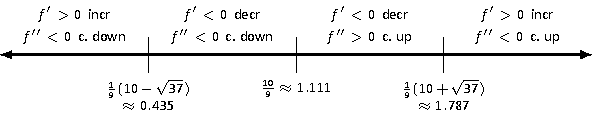
\includegraphics[scale=.75]{figures/figsketchline1}
\end{center}

\item We plot the appropriate points on axes as shown in Figure~\ref{fig:sketch1}-(a) and connect the points with straight lines. In Figure~\ref{fig:sketch1}-(b) we adjust these lines to demonstrate the proper concavity. Our curve crosses the $y$ axis at $y=5$ and crosses the $x$ axis near $x=-0.424$. In Figure~\ref{fig:sketch1}-(c) we show a graph of $f$ drawn with a computer program, verifying the accuracy of our sketch.
\end{enumerate}
\end{example} % EXAMPLE

\begin{example} \label{Ex:3.2.Eg5}
Sketch $\ds f(x) = \frac{x^2-x-2}{x^2-x-6}$.

\solution We follow the steps outlined in the Curve Sketching Concept.

\begin{enumerate}[1)]
\item In determining the domain, we assume it is all real numbers and looks for restrictions. We find that at $x=-2$ and $x=3$, $f(x)$ is not defined. So the domain of $f$ is $D = \{\text{real numbers } x\ | \ x\neq -2,3\}$.

\item To find the critical values of $f$, we first find $f'(x)$. Using the Quotient Rule, we find 
$$f'(x) = \frac{-8x+4}{(x^2+x-6)^2} = \frac{-8x+4}{(x-3)^2(x+2)^2}.$$
		
We find that $\fp(x) = 0$ when $x = 1/2$, and $\fp$ is undefined when $x=-2,3$. 
		
\item To find the possible points of inflection, we find $\fpp(x)$, again employing the Quotient Rule: 
$$\fpp(x) = \frac{24x^2-24x+56}{(x-3)^3(x+2)^3}.$$
		
We find that $\fpp(x)$ is never $0$ (setting the numerator equal to $0$ and solving for $x$, we find the only roots to this quadratic are complex) and $\fpp$ is undefined when $x=-2,3$. Thus concavity will possibly only change at $x=-2$ and $x=3$.
		
\item The vertical asymptotes of $f$ are at $x=-2$ and $x=3$, the places where $f$ is undefined.
		
\item There is a horizontal asymptote of $y=1$, as $\ds \lim_{x\to -\infty}f(x) = 1$ and $\ds\lim_{x\to\infty}f(x) =1$.
		
\item We place the values $x=1/2$, $x=-2$ and $x=3$ on a number line as shown below. We mark in each interval whether $f$ is increasing or decreasing, concave up or down. We see that $f$ has a relative maximum at $x=1/2$; concavity changes only at the vertical asymptotes.

\begin{center}
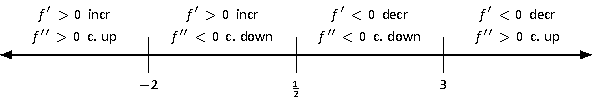
\includegraphics[scale=.75]{figures/figsketchline2}
\end{center}

\item In Figure~\ref{fig:sketch2}-(a), we plot the points from the number line on a set of axes and connect the points with straight lines to get a general idea of what the function looks like (these lines effectively only convey increasing/decreasing information). 

In Figure~\ref{fig:sketch2}-(b), we adjust the graph with the appropriate concavity. We also show $f$ crossing the $x$ axis at $x=-1$ and $x=2$.

Figure~\ref{fig:sketch2}-(c) shows a computer generated graph of $f$, which verifies the accuracy of our sketch.
\end{enumerate}
\end{example}

\begin{marginfigure}[-16cm] % MARGIN FIGURE
%\captionsetup[subfigure]{labelformat=empty}
\subfloat[]{\margingraphics{figures/figsketch2a}}

\subfloat[]{\margingraphics{figures/figsketch2b}}

\subfloat[]{\margingraphics{figures/figsketch2}}
\caption{Sketching $f$ in Example~\ref{Ex:3.2.Eg5}.}
\label{fig:sketch2}
\end{marginfigure} % EXAMPLE

\begin{example} \label{Ex:3.2.Eg7}
Sketch $\ds f(x) = \frac{5(x-2)(x+1)}{x^2+2x+4}.$

\solution We again follow the steps outlined in the Curve Sketching Concept.
\begin{enumerate}[1)]
\item We assume that the domain of $f$ is all real numbers and consider restrictions. The only restrictions come when the denominator is 0, but this never occurs. Therefore the domain of $f$ is all real numbers, $\mathbb{R}$.
\item We find the critical values of $f$ by setting $\fp(x)=0$ and solving for $x$. We find 
$$\fp(x) = \frac{15x(x+4)}{(x^2+2x+4)^2} \quad \Rightarrow \quad \fp(x) = 0 \text{ when } \ x=-4,0.$$
\item We find the possible points of inflection by solving $\fpp(x) = 0$ for $x$. We find
$$\fpp(x) = -\frac{30x^3+180x^2-240}{(x^2+2x+4)^3} .$$ The cubic in the numerator does not factor very ``nicely.'' We instead approximate the roots at $x= -5.759$, $x=-1.305$ and $x=1.064$.
			
\item There are no vertical asymptotes.
\item We have a horizontal asymptote of $y=5$, as $\ds \lim_{x\to-\infty}f(x) = \lim_{x\to\infty}f(x) = 5$.
\item We place the critical points and possible points on a number line as shown below and mark each interval as increasing/decreasing, concave up/down appropriately.
	
\begin{center}
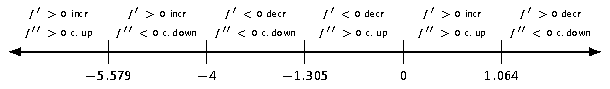
\includegraphics[scale=.75]{figures/figsketchline3}
\end{center}
	
\item In Figure~\ref{fig:sketch3}-(a) we plot the significant points from the number line as well as the two roots of $f$, $x=-1$ and $x=2$, and connect the points with straight lines to get a general impression about the graph. In Figure~\ref{fig:sketch3}-(b), we add concavity. Figure~\ref{fig:sketch3}-(c) shows a computer generated graph of $f$, affirming our results.		
\end{enumerate}
\end{example}

\begin{marginfigure}[-4cm] % MARGIN FIGURE
%\captionsetup[subfigure]{labelformat=empty}
\subfloat[]{\margingraphics{figures/figsketch3a}}

\subfloat[]{\margingraphics{figures/figsketch3b}}

\subfloat[]{\margingraphics{figures/figsketch3}}
\caption{Sketching $f$ in Example~\ref{Ex:3.2.Eg7}.}
\label{fig:sketch3}
\end{marginfigure} % EXAMPLE

In each of our examples, we found significant points on the graph of $f$ that corresponding to changes in increasing/decreasing or concavity. We connected these points with straight lines, then adjusted for concavity, and finished by showing a very accurate, computer generated graph.

Why are computer graphics so good? It is not because computers are ``smarter'' than we are. Rather, it is largely because computers are much faster at computing than we are. In general, computers graph functions much like most students do when first learning to draw graphs: they plot equally spaced points, then connect the dots using lines. By using lots of points, the connecting lines are short and the graph looks smooth. 

This does a fine job of graphing in most cases (in fact, this is the method used for many graphs in this text). However, in regions where the graph is very ``curvy,'' this can generate noticeable sharp edges on the graph unless a large number of points are used. High quality computer algebra systems, such as \textit{Mathematica}, use special algorithms to plot lots of points only where the graph is ``curvy.''

In Figure~\ref{fig:mathematica_sinx}, a graph of $y=\sin(x)$ is given, generated by \textit{Mathematica}. The small points represent each of the places \textit{Mathematica} sampled the function. Notice how at the ``bends'' of $\sin(x)$, lots of points are used; where $\sin(x)$ is relatively straight, fewer points are used. (Many points are also used at the endpoints to ensure the ``end behavior'' is accurate.) 

\begin{marginfigure} % MARGIN FIGURE
\margingraphics{figures/figmathematica_sinx}
\caption{A graph of $y=\sin(x)$ generated by \textit{Mathematica}.}\label{fig:mathematica_sinx}
\end{marginfigure}

How does \textit{Mathematica} know where the graph is ``curvy''? Calculus. When we study \textit{curvature} in multivariate calculus, we will see how the first and second derivatives of a function work together to provide a measurement of ``curviness.'' \textit{Mathematica} employs algorithms to determine regions of ``high curvature'' and plots extra points there.

%-------------------------------------------------------
% SUMMARY
%-------------------------------------------------------
\begin{summary}
\item The critical values of a continuous function $f$ are the values of $p$ for which $f'(p) = 0$ or $f'(p)$ does not exist.  These values are important because they identify horizontal tangent lines or corner points on the graph, which are the only possible locations at which a local maximum or local minimum can occur.
\item Given a differentiable function $f$, whenever $f'$ is positive, $f$ is increasing; whenever $f'$ is negative, $f$ is decreasing.  The first derivative test tells us that at any point where $f$ changes from increasing to decreasing, $f$ has a local maximum, while conversely at any point where $f$ changes from decreasing to increasing $f$ has a local minimum.
\item Given a twice differentiable function $f$, if we have a horizontal tangent line at $x = p$ and $f''(p)$ is nonzero, then the fact that $f''$ tells us the concavity of $f$ will determine whether $f$ has a maximum or minimum at $x = p$.  In particular, if $f'(p) = 0$ and $f''(p) < 0$, then $f$ is concave down at $p$ and $f$ has a local maximum there, while if $f'(p) = 0$ and $f''(p) > 0$, then $f$ has a local minimum at $p$.  If $f'(p) = 0$ and $f''(p) = 0$, then the second derivative does not tell us whether $f$ has a local extreme at $p$ or not.
\end{summary}

\clearpage

%--------------
% EXERCISES
%--------------
\begin{adjustwidth*}{}{-2.25in}
\textbf{{\large Exercises}}
\setlength{\columnsep}{25pt}
\begin{multicols*}{2}
\noindent Terms and Concepts \small
\begin{enumerate}[1)]
\item In your own words describe what it means for a function to be increasing.
\item What does a decreasing function ``look like''?
\item Sketch a graph of a function on $[0,2]$ that is increasing but not strictly increasing.
\item Give an example of a function describing a situation where it is ``bad'' to be increasing and ``good'' to be decreasing.
\item A function $f$ has derivative $\fp(x) = (\sin(x)+2)e^{x^2+1}$, where $\fp(x) >1 $ for all $x$. Is $f$ increasing, decreasing, or can we not tell from the given information?
\item Sketch a graph of a function $f(x)$ that is:
	\ba
	\item		Increasing, concave up on $(0,1)$,
	\item		increasing, concave down on $(1,2)$,
	\item		decreasing, concave down on $(2,3)$ and 
	\item		increasing, concave down on $(3,4)$.
	\ea
\item Is is possible for a function to be increasing and concave down on $(0,\infty)$ with a horizontal asymptote of $y=1$? If so, give a sketch of such a function.
\item Is is possible for a function to be increasing and concave up on $(0,\infty)$ with a horizontal asymptote of $y=1$? If so, give a sketch of such a function.
\end{enumerate} 

\noindent {\normalsize Problems} \small

\noindent{\bf In exercises 9--18, a function is given.
\ba
\item Find the critical numbers of $f$.
\item Determine the intervals on which $f$ is increasing and decreasing.
\item Use the First Derivative Test to determine whether each critical point is a local maximum, local minimum, or neither.
\item Use the Second Derivative Test to determine whether each critical point is a local maximum, local minimum, or if the test fails.
\ea}

\begin{enumerate}[1),resume]
\item $\ds f(x) =x^2+2x-3$
	
\item $\ds f(x) =x^3+3x^2+3$
	
\item $\ds f(x) =2 x^3+x^2-x+3$

\item $\ds f(x) =x^3-3x^2+3x-1$

\item $\ds f(x) =\frac{1}{x^2-2x+2}$

\item $\ds f(x) =\frac{x^2-4}{x^2-1}$

\item $\ds f(x) =\frac{x}{x^2-2x-8}$

\item $\ds f(x) =\frac{(x-2)^{2/3}}{x}$

\item $\ds f(x) =\sin x\cos x$ on $(-\pi,\pi)$

\item $\ds f(x) =x^5-5x$
\end{enumerate}

\noindent{\bf In exercises 19--31, a function is given.
\ba
\item Find the possible points of inflection of $f$.
\item Determine the intervals on which $f$ is concave up and concave down.
\item Determine whether each possible point of inflection is in fact a point of inflection.
\ea}

\begin{enumerate}[1),resume]
\item $\ds f(x) = x^2-2x+1$ \label{exer:03_04_ex_16}
\item $\ds f(x) = -x^2-5x+7$
\item $\ds f(x) = x^3-x+1$
\item $\ds f(x) = 2x^3-3x^2+9x+5$
\item $\ds f(x) = \frac{x^4}{4}+\frac{x^3}{3}-2 x+3$
\item $\ds f(x) = -3 x^4+8 x^3+6 x^2-24 x+2$
\item $\ds f(x) = x^4-4x^3+6x^2-4x+1$
\item $\ds f(x) = \frac{1}{x^2+1}$
\item $\ds f(x) = \frac{x}{x^2-1}$
\item $\ds f(x) = \sin x + \cos x$ on $(-\pi,\pi)$
\item $\ds f(x) = x^2e^x$
\item $\ds f(x) = x^2\ln x$
\item $\ds f(x) = e^{-x^2}$\label{exer:03_04_ex_28}
\end{enumerate}

\noindent{\bf In exercises 32--45, sketch a graph of the given function using the steps outlined in the Curve Sketching Concept.}

\begin{enumerate}[1),resume]
\item $\ds f(x) = x^3-2x^2+4x+1$
\item $\ds f(x) = -x^3+5x^2-3x+2$
\item $\ds f(x) = x^3+3x^2+3x+1$
\item $\ds f(x) = x^3-x^2-x+1$
\item $\ds f(x) = (x-2)\ln (x-2)$
\item $\ds f(x) = (x-2)^2\ln (x-2)$
\item $\ds f(x) = \frac{x^2-4}{x^2}$
\item $\ds f(x) = \frac{x^2-4x+3}{x^2-6x+8}$
\item $\ds f(x) = \frac{x^2-2x+1}{x^2-6x+8}$
\item $\ds f(x) = x\sqrt{x+1}$
\item $\ds f(x) = x^2e^x$
\item $\ds f(x) = \sin x \cos x$ on $[-\pi,\pi]$
\item $\ds f(x) = (x-3)^{2/3} + 2$
\item $\ds f(x) = \frac{(x-1)^{2/3}}{x}$
\end{enumerate}

%------------------------------------------
% END OF EXERCISES ON FIRST PAGE
%------------------------------------------
\end{multicols*}
\end{adjustwidth*}

%\clearpage
%
%\begin{adjustwidth*}{}{-2.25in}
%\setlength{\columnsep}{25pt}
%\begin{multicols*}{2}\small
%
%\begin{enumerate}[1),start=12]
%
%\item \label{exer:04_02_ex_12}A rope, attached to a weight, goes up through a pulley at the ceiling and back down to a worker. The man holds the rope at the same height as the connection point between rope and weight.
%
%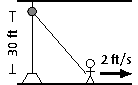
\includegraphics[scale=1.25]{figures/fig04_02_ex_12}
%
%Suppose the man stands directly next to the weight (i.e., a total rope length of 60 ft) and begins to walk away at a rate of 2ft/s. How fast is the weight rising when the man has walked:
%\begin{enumerate}
%\item	10 feet?
%\item	40 feet?
%\end{enumerate}
%How far must the man walk to raise the weight all the way to the pulley?
%
%\item Consider the situation described in Exercise \ref{exer:04_02_ex_12}. Suppose the man starts 40ft from the weight and begins to walk away at a rate of 2ft/s. 
%\begin{enumerate}
%\item	How long is the rope?
%\item	How fast is the weight rising after the man has walked 10 feet?
%\item	How fast is the weight rising after the man has walked 40 feet?
%\item	How far must the man walk to raise the weight all the way to the pulley?
%\end{enumerate}
%
%\item A company that produces landscaping materials is dumping sand into a conical pile. The sand is being poured at a rate of 5ft$^3$/sec; the physical properties of the sand, in conjunction with gravity, ensure that the cone's height is roughly 2/3 the length of the diameter of the circular base. 
%
%How fast is the cone rising when it has a height of 30 feet?
%
%\item A baseball diamond is a square with sides 90 feet long.  Suppose a baseball player is advancing from second to third base at the rate of 24 feet per second, and an umpire is standing on home plate.  Let  $\theta$ be the angle between the third baseline and the line of sight from the umpire to the runner.  How fast is $\theta$ changing when the runner is 30 feet from third base?
%	
%\item Sand is being dumped off a conveyor belt onto a pile in such a way that the pile forms in the shape of a cone whose radius is always equal to its height.  Assuming that the sand is being dumped at a rate of 10 cubic feet per minute, how fast is the height of the pile changing when there are 1000 cubic feet on the pile?
%	
%\item A swimming pool is 60 feet long and 25 feet wide. Its depth varies uniformly from 3 feet at the shallow end to 15 feet at the deep end, as shown below.
%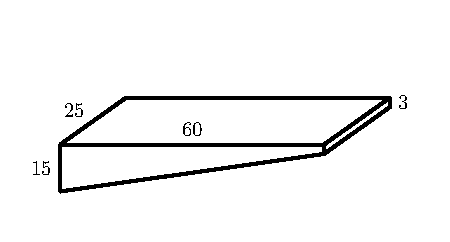
\includegraphics{figures/3_5_Ez3.eps}
%Suppose the pool has been emptied and is now being filled with water at a rate of 800 cubic feet per minute. At what rate is the depth of water (measured at the deepest point of the pool) increasing when it is 5 feet deep at that end?  Over time, describe how the depth of the water will increase:  at an increasing rate, at a decreasing rate, or at a constant rate.  Explain.
%
%\end{enumerate}
%
%%---------------------------------------------
%% END OF EXERCISES ON SECOND PAGE
%%---------------------------------------------
%\end{multicols*}
%\end{adjustwidth*}

\afterexercises 

\cleardoublepage